\section{Week 3: Document representation and matching}
\subsection{Query analysis}

\begin{minipage}{.5\textwidth}
\textbf{Pipeline}: should be the same as document processing pipeline.
\begin{itemize}
    \setlength\itemsep{0em}
    \item Normalization
    \item Spelling correction
    \item Segmentation
    \item Stemming
    \item Term expansion, etc..
\end{itemize}
\end{minipage}
\begin{minipage}{.45\textwidth}
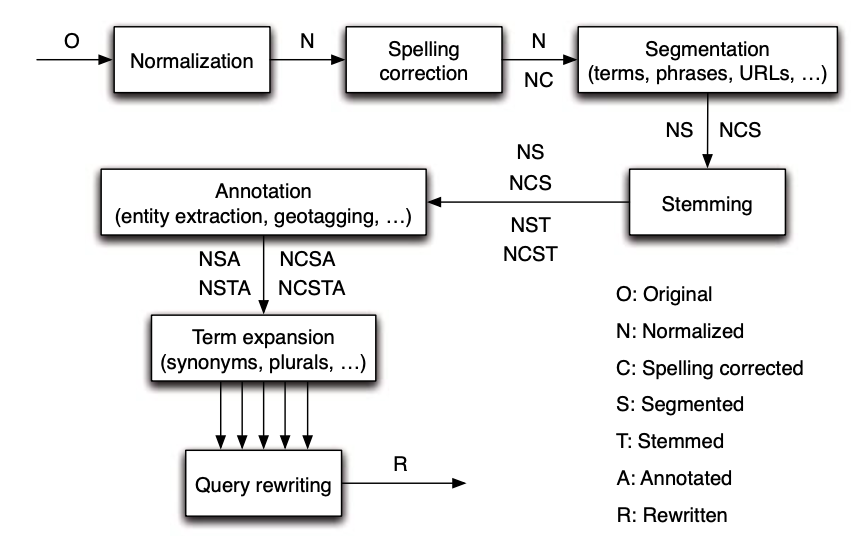
\includegraphics[scale=0.5]{figures/query-analysis.png}
\end{minipage}

\subsection{Query processing}
\begin{minipage}{.5\textwidth}
\textbf{Practical considerations}:
\begin{itemize}
    \setlength\itemsep{0em}
    \item Conjunctive mode (AND)
    \item Document-at-a-time
    \item A score is usually computed as a linear combination of query-dependent and query-independent scores
\end{itemize}
\end{minipage}
\begin{minipage}{.45\textwidth}
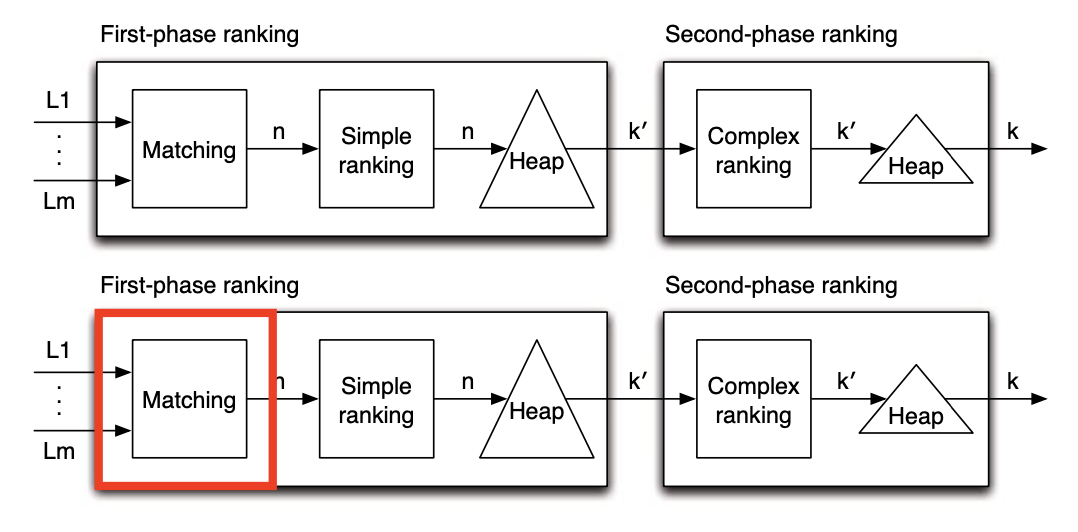
\includegraphics[scale=0.4]{figures/query-processing.png}
\end{minipage}

\subsection{Termbased Retrieval}
\begin{enumerate}
    \item \textbf{Vector space model}
    \begin{itemize}
    \setlength\itemsep{0em}
        \item \textcolor{Maroon}{Document as vector}: \textcolor{MidnightBlue}{binary occurrence} of a term in a document (each document is a vector)
        \item \textcolor{Maroon}{Match using Cosine similarity}
        $$ 
        \begin{aligned}
        \operatorname{sim}(d, q)=\cos (\vec{v}(d), \vec{v}(q)) &=\frac{\vec{v}(d) \cdot \vec{v}(q)}{\|\vec{v}(d)\| \cdot\|\vec{v}(q)\|} 
        =\frac{\sum_{i=1}^{|V|} d_{i} \cdot q_{i}}{\sqrt{\sum_{i=1}^{|V|} d_{i}^{2}} \cdot \sqrt{\sum_{i=1}^{|V|} q_{i}^{2}}}
        \end{aligned} 
        $$
        Where: V is the size of the vocabulary.
        \item \textbf{\textcolor{Maroon}{Instead}} of using the \textcolor{MidnightBlue}{binary occurrence}, we can use these weights:
        \begin{itemize}
            \item \textbf{\textcolor{Fuchsia}{Term frequency}}:
            \begin{itemize}
                \item{\makebox[5cm]{\textcolor{Fuchsia}{Raw term frequency}:\hfill} $tf(t, d)$}
                \item{\makebox[5cm]{\textcolor{Fuchsia}{Long term frequency}:\hfill} $\begin{cases}1+\log t f(t, d) & \text { if } t f(t, d)>0 \\ 0 & \text { otherwise }\end{cases}$}
            \end{itemize}
            \item \textbf{\textcolor{RedOrange}{TF-IDF}}:
            \begin{itemize}
                \item{\makebox[6cm]{\textcolor{ForestGreen}{Inverse document frequency (1)}:\hfill} $idf(t) = \log \frac{N}{df(t)}$} 
                \item{\makebox[6cm]{\textcolor{ForestGreen}{Inverse document frequency (2)}:\hfill} $\max \left\{0, \log \frac{N-d f(t)}{d f(t)}\right\}$} \\
                \textbf{Where}:
                $$
                \begin{aligned}
                    &df(t) &= \;\;\; &\text{document frequency of term t} \\
                    &N &= \;\;\; &\text{total number of documents in a collection}
                \end{aligned}
                $$
                \item \textbf{\textcolor{RedOrange}{TF-IDF}}:
                $$
                \text{\textcolor{RedOrange}{TF-IDF}}(t,d) = \text{\textcolor{Fuchsia}{tf}}(t,d) \cdot \text{\textcolor{ForestGreen}{idf}}(t)
                $$
            \end{itemize}
        \end{itemize}
    \end{itemize}
    \item \textbf{Language modelling (LM) in IR}:
    \begin{itemize}
        \item \textbf{\textcolor{Maroon}{Method}} \\
        \textbf{Statistical language model} is a probability distr. over sequences of words.
        \begin{itemize}
            \item given a \textbf{sequence} of \textbf{length m}
            \item a LM assigns probability $P(w_1, \cdots, w_m)$ to this sequence 
            \vspace{0.2cm}
            \item{\makebox[3cm]{Unigram LM:\hfill} $P(w_1, \cdots, w_m) = P(w_1) \cdots P(w_m)$}
            \item{\makebox[3cm]{Bi-gram LM:\hfill} $P\left(w_{1}, \ldots, w_{m}\right)=P\left(w_{1}\right) P\left(w_{2} \mid w_{1}\right) \ldots P\left(w_{m} \mid w_{m-1}\right)$}
            \item Documents as distributions (1):
            \begin{itemize}
                \item{\makebox[5cm]{\textbf{Unigram LM}:\hfill} $P\left(t \mid M_{d}\right)=\frac{t f(t, d)}{d l(d)}$}
                \item $d l(d)$ is total number of terms in the document (length of document)
                \item this is the \textcolor{Maroon}{maximum likelihood estimation}
                \item a document is a multinomial distribution over words
                \item if some vocabulary terms do not in document d, then $P(t \mid M_d) = 0$
                \item addressed by \textcolor{Maroon}{smoothing}
            \end{itemize}
            \item How to match the distributions (using query likelihood model QLM) (2)?
            \begin{itemize}
                \item{\makebox[7cm]{\textbf{Likelihood} of a doc given a query:\hfill} $P(d \mid q)=\frac{P(q \mid d) P(d)}{P(q)}$}
                \vspace{0.15cm}
                \item \textbf{Prior distr.} over queries P(q) does  \\
                \makebox[7cm]{  \textcolor{Maroon}{not affect} matching a particular query: \hfill}
                $P(d \mid q) \stackrel{\text { rank }}{=} P(q \mid d) P(d)$
                \item Usually, the \textbf{prior distr} over docs P(d) \\
                \makebox[6cm]{  is assumed to be \textcolor{Maroon}{uniform}: \hfill}
                $P(d \mid q) \stackrel{r a n k}{=} P(q \mid d)=P\left(q \mid M_{d}\right)$
                \item \textcolor{Maroon}{"Bag of words"} assumption: \\
                \makebox[5cm]{  terms are \textcolor{Maroon}{independent}: \hfill}
                $P\left(q \mid M_{d}\right)=\prod_{t \in q} P\left(t \mid M_{d}\right)=\prod_{t \in q} \frac{t f(t, d)}{d l(d)}$
                \item Match using \textbf{\textcolor{Maroon}{KL-divergence}}
                $$ K L\left(M_{d} \| M_{q}\right)=\sum_{t \in V} P\left(t \mid M_{q}\right) \log \frac{P\left(t \mid M_{q}\right)}{P\left(t \mid M_{d}\right)} $$
            \end{itemize}
        \end{itemize}
        \item \textbf{\textcolor{Maroon}{Smoothing}} (3)
        \begin{itemize}
            \item \textbf{\textcolor{Emerald}{Jelinek-Mercer smoothing}}
            $$ 
            \begin{aligned}
            P_{s}\left(t \mid M_{d}\right) &=\lambda P\left(t \mid M_{d}\right)+(1-\lambda) P\left(t \mid M_{c}\right) \\
            &=\lambda \frac{t f(t, d)}{d l(d)}+(1-\lambda) \frac{c f(t)}{c l}
            \end{aligned}
            $$
            \textbf{Where}:
                \makebox[7cm]{$cf(t)$ = \text{collection frequency of term t}} \\
                \makebox[7.2cm]{ $cl$ = \text{collection length}}
            \item \textbf{\textcolor{DarkOrchid}{Dirichlet smoothing}}
            \begin{itemize}
                \item A \textbf{unigram language model} can be seen as a \textcolor{DarkOrchid}{multinomial distr.} over words $\mathcal{L}_{d}\left(n_{1}, \ldots, n_{k} \mid p_{1}, \ldots, p_{k}\right)$:
                \vspace{0.1cm}
                \begin{itemize}
                    \item[$\circ$] $n_i = tf(t_i, d)$
                    \item[$\circ$] $p_i = P(t_i \mid M_d)$ \\
                \end{itemize}
                \item The \textbf{conjugate prior} for \textbf{multinomial} is the \textcolor{DarkOrchid}{Dirichlet distr.} \\ $P_{\text {prior }}\left(p_{1}, \ldots, p_{k} ; \alpha_{1}^{p r}, \ldots, \alpha_{k}^{p r}\right)$:
                \\
                \begin{itemize}
                    \item[$\circ$] $\alpha_{i}^{p r}=\mu P\left(t_{i} \mid M_{c}\right)$ 
                    \item[$\circ$] $\mu \text { is a smoothing parameter }\left(\lambda=\frac{d l}{d l+\mu}\right)$ 
                \end{itemize}
                \item The \textbf{posterior} is the \textcolor{DarkOrchid}{Dirichlet distr.} with parameters  $$\alpha_{i}^{p o}=n_{i}+\alpha_{i}^{p r}=\operatorname{tf}\left(t_{i}, d\right)+\mu P\left(t_{i} \mid M_{c}\right)$$
                \item \textbf{\textcolor{DarkOrchid}{Dirichlet smoothing}}:
                $$
                P_{s}\left(t \mid M_{d}\right)=\frac{t f\left(t_{i}, d\right)+\mu P\left(t_{i} \mid M_{c}\right)}{d l(d)+\mu}
                $$
            \end{itemize}
        \end{itemize}
    \end{itemize}
    \item \textbf{BM25}
    $$
    B M 25=\sum_{t \in q} \log \left[\frac{N}{d f(t)}\right] \cdot \frac{\left(k_{1}+1\right) \cdot t f(t, d)}{k_{1} \cdot\left[(1-b)+b \cdot \frac{d l(d)}{d l_{a v g}}\right]+t f(t, d)}
    $$
    \\
    \begin{minipage}{0.35\textwidth}
        \begin{itemize}
            \setlength\itemsep{0em}
            \item $k_{1}, b$ - parameters
            \item $d l(d)$ - length doc $d$
            \item $d l_{a v g}-$ avg. doc length
            \\
        \end{itemize}
    \end{minipage}
    \begin{minipage}{0.65\textwidth}
        \begin{itemize}
            \setlength\itemsep{0em}
            \item[--] $k_{1} = 0 \rightarrow $ summation of idfs 
            \item[--] $k_{1} = \infty \rightarrow $ summation of tf-idfs
            \item[--] $b = 0 \rightarrow $ no normalization by doc length 
            \item[--] $b = 1 \rightarrow $ doc length full effect
            \item[--] $tf \rightarrow $ compensates (if it's too large for example)
        \end{itemize}
    \end{minipage}
    
    \textbf{BM25 for \textcolor{Maroon}{long queries}} 
    $$
    B M 25=\sum_{t \in q} \log \left[\frac{N}{d f(t)}\right] \cdot \frac{\left(k_{1}+1\right) \cdot t f(t, d)}{k_{1} \cdot\left[(1-b)+b \cdot \frac{d l(d)}{d l_{a v g}}\right]+t f(t, d)} \textcolor{Maroon}{\cdot \frac{\left(k_{3}+1\right) t f(t, q)}{k_{3}+t f(t, q)}}
    $$
\end{enumerate}

\subsection{Semantic-based Retrieval}
\begin{enumerate}
    \setlength\itemsep{0em}
    \item \textbf{Topic modelling}  \\
    \textbf{\textcolor{Maroon}{Unigram language model}} \\
    \begin{minipage}{0.3\textwidth}
        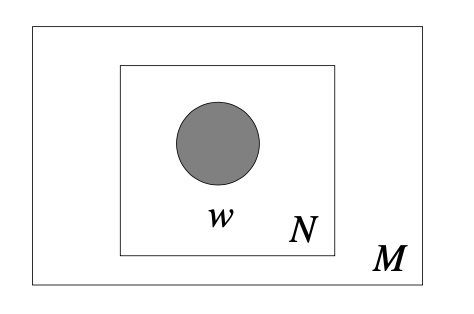
\includegraphics[scale=0.5]{figures/uni1.png}
    \end{minipage}
    \begin{minipage}{0.2\textwidth}
        $$
        \begin{aligned}
        &W_{ij} \sim \operatorname{Mult}(d_i) \\
        &i \in \{1, \cdots, M\} \\
        &j \in \{1, \cdots, N_i\} \\
        & \\
        \end{aligned}
        $$
    \end{minipage}
    \begin{minipage}{0.5\textwidth}
        \begin{itemize}
            \setlength\itemsep{0em}
            \item[--] The circle is a \textcolor{Maroon}{random variable}.
            \item[--] Shaded circle is observed, empty is not observed.
            \item[--] \textcolor{Maroon}{RV} is occurrence of word
        \end{itemize}
    \end{minipage}
    
    \textbf{So}: we have a collection of M documents, each document has a length of N. On every $n$th position the word w may either occur or not.
    \\
    \\
    \textbf{\textcolor{MidnightBlue}{Mixture of unigrams}} \\
    \begin{minipage}{0.3\textwidth}
        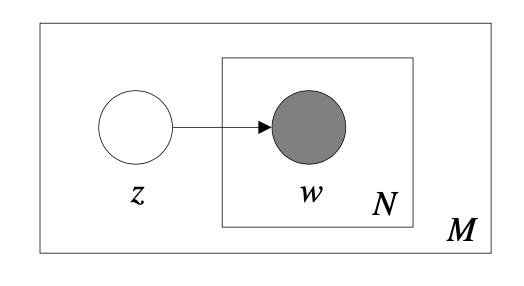
\includegraphics[scale=0.5]{figures/uni2.png}
    \end{minipage}
    \begin{minipage}{0.2\textwidth}
        $$
        \begin{aligned}
        z_{i} & \sim \operatorname{Mult}(\theta) \\
        w_{i j} & \sim \operatorname{Mult}\left(\phi_{z_{i}}\right) \\
        &
        \end{aligned}
        $$
    \end{minipage}
    \begin{minipage}{0.5\textwidth}
        \;\;\; 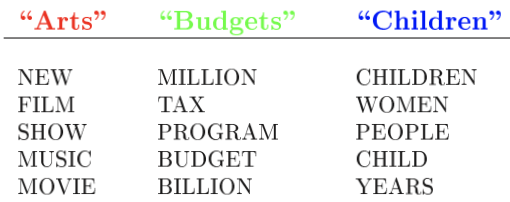
\includegraphics[scale=0.6]{figures/mixture.png}
    \end{minipage}
    
    \textbf{This time}: we first added an unobserved hidden variable $z$ (topic). Now we pick a topic M times. From that topic we sample N times. Topics are for example as depicted in the right figure above: "arts", "budgets" and "children".  
    \\
    \\
    \textbf{\textcolor{Bittersweet}{Probabilistic latent semantic analysis (pLSA)}} \\
    \begin{minipage}{0.3\textwidth}
        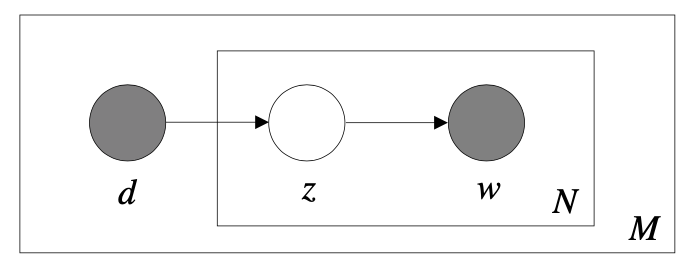
\includegraphics[scale=0.3]{figures/uni3.png}
    \end{minipage}
    \begin{minipage}{0.2\textwidth}
        $$
        \begin{aligned}
        z_{ij} & \sim \operatorname{Mult}(\theta_i) \\
        w_{i j} & \sim \operatorname{Mult}\left(\phi_{z_{ij}}\right) \\
        &
        \end{aligned}
        $$
    \end{minipage}
    \begin{minipage}{0.5\textwidth}
        \;\;\; 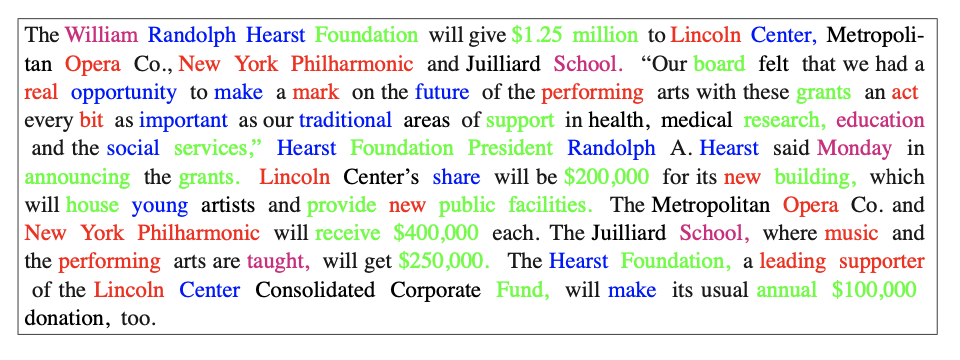
\includegraphics[scale=0.4]{figures/plsa.png}
    \end{minipage}
    
    \textbf{In this case}: we assume that every word in the document comes from a \textcolor{Bittersweet}{certain topic}. The document is observed and we have M documents. For every position in the document (that is observed) we randomly sample a topic from the multinomal distr. (which is not known). From that topic we sample a word. \\
    \\
    So the \textbf{probability of a word given a document}:
    $$
    P(w \mid d)=\sum_{z} P\left(w \mid \phi_{z}\right) P\left(z \mid \theta_{d}\right)
    $$
    
    This is \textbf{\textcolor{ForestGreen}{better}} than before, because we are semantically matching. \textcolor{Red}{Before} we were matching exactly (terms in a query and terms in a document). If the query term did not occur in the document, we used smoothing. \textbf{\textcolor{ForestGreen}{Now}}, even if the query term does not occur in the document, but the document is in general about the topic of the query, we still want this document to be ranked \textbf{high}.
    
    \textbf{\textcolor{OliveGreen}{Latent Dirichlet allocation (LDA)}} \\
    \\
    \begin{minipage}{0.4\textwidth}
        \;\;\; 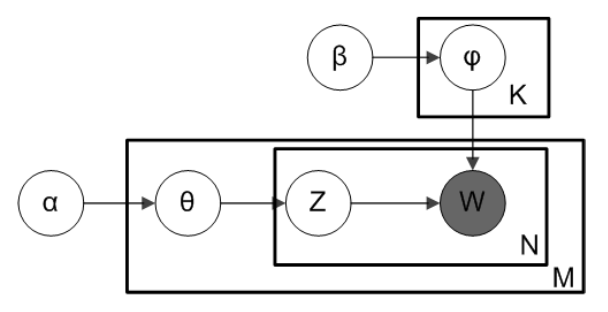
\includegraphics[scale=0.5]{figures/LDA.png}
    \end{minipage}
    \begin{minipage}{0.6\textwidth}
    \begin{enumerate}
        \item Choose $\theta_{i} \sim \operatorname{Dir}(\alpha)$, where $i \in\{1, \ldots, M\}$
        \item Choose $\phi_{k} \sim \operatorname{Dir}(\beta)$, where $k \in\{1, \ldots, K\}$
        \item For each position $j$, where $j \in\left\{1, \ldots, N_{i}\right\}$
        \begin{enumerate}
            \item Choose a topic $z_{i j} \sim \operatorname{Mult}\left(\theta_{i}\right)$
            \item Choose a word $w_{i j} \sim \operatorname{Mult}\left(\phi_{z_{i j}}\right)$
        \end{enumerate}
    \end{enumerate}
    \end{minipage}
    \\
    \\
    \textbf{This one} is basically the same as pLSA, but with priors added. 
    \\
    \\
    \textbf{Estimating LDA}: expectation-maximization \textbf{\textcolor{Maroon}{$[$BEYOND IR1!!$]$}} \\
    \begin{itemize}
        \item \textbf{E-step}: define the expected value of the log-likelihood function, with respect to the current estimates of the parameters $\boldsymbol{\theta}^{(t)}, \boldsymbol{\phi}^{(t)}:$
        $$ Q\left(\boldsymbol{\theta}, \boldsymbol{\phi} \mid \boldsymbol{\theta}^{(t)}, \boldsymbol{\phi}^{(t)}\right)=\mathrm{E}_{\mathrm{Z} \mid \mathrm{W}, \boldsymbol{\theta}^{(t)}, \phi^{(t)}}[\log L(\boldsymbol{\theta}, \boldsymbol{\phi} ; \mathrm{W}, \mathrm{Z})] $$
        \item \textbf{M-step}: find the parameters that maximize this quantity
        $$ 
        \boldsymbol{\theta}^{(t+1)}, \boldsymbol{\phi}^{(t+1)}=\underset{\boldsymbol{\theta}, \boldsymbol{\phi}}{\arg \max } Q\left(\boldsymbol{\theta}, \boldsymbol{\phi} \mid \boldsymbol{\theta}^{(t)}, \boldsymbol{\phi}^{(t)}\right)
        $$
        \item Repeat until convergence
    \end{itemize}
    \item \textbf{Latent semantic indexing/analysis}
    \begin{itemize}
        \item \textbf{Singular Value Decomposition (SVD)} \\
        \begin{minipage}{0.5\textwidth}
            \begin{itemize}
                \setlength\itemsep{0em}
                \item \textcolor{Maroon}{$C$} $=U\Sigma V^T$: $m \times n$ (term document) 
                \item \textcolor{Maroon}{$U$}: $m \times m$ unitary matrix 
            \end{itemize}
        \end{minipage}
        \begin{minipage}{0.5\textwidth}
            \begin{itemize}
                \setlength\itemsep{0em}
                \item \textcolor{Maroon}{$\Sigma$}: diag. $m \times n$ with singular values 
                \item \textcolor{Maroon}{$V^T$}: $n \times n$ unitary matrix
            \end{itemize}
        \end{minipage}
        
        \item \textbf{Low-rank approximation}
        $$
        \begin{aligned}
        C &=U \Sigma V^{T}=\sum_{i=1}^{\min (m, n)} \sigma_{i} \vec{u}_{i} \vec{v}_{i}^{T} 
         \approx \sum_{i=1}^{k} \sigma_{i} \vec{u}_{i} \vec{v}_{i}^{T}=U_{k} \Sigma_{k} V_{k}^{T}
        \end{aligned}
        $$
        \item \textbf{Latent semantic indexing/analysis} \\
        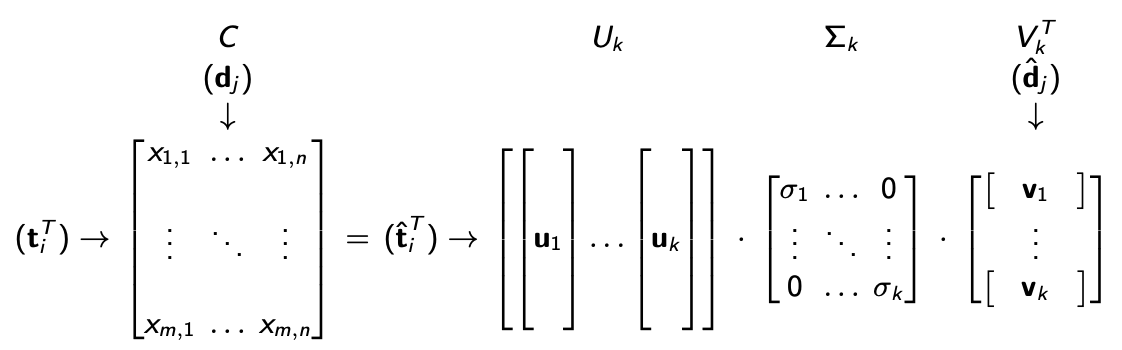
\includegraphics[scale=0.6]{figures/lsa.png}
        
        $$ d_{j}=U_{k} \Sigma_{k} \hat{d}_{j} \Longrightarrow \hat{d}_{j}=\Sigma_{k}^{-1} U_{k}^{T} d_{j} $$
        
        \item \textbf{Documents as vectors}:
        \begin{itemize}
            \item Given a collection of documents, perform SVD and low-rank approximation to obtain $\Sigma_k$ and $U_k$
            \item Given a document and a query, represent them as a vectors in the obtained “semantic” vector space \;\;
            $
            \hat{d}=\Sigma_{k}^{-1} U_{k}^{T} d \;\;\;\;\;\;
            \hat{q}=\Sigma_{k}^{-1} U_{k}^{T} q
            $
            \item Match the obtained “semantic” vector representations $\hat{d}$ and $\hat{q}$ using cosine similarity
        \end{itemize}
        
    \end{itemize}
    \item \textbf{Neural models}
    \begin{itemize}
        \item \textbf{\textcolor{Maroon}{Word embeddings}} \\
        \\
        \begin{minipage}{0.5\textwidth}
        \textbf{Word2Vec} \\
            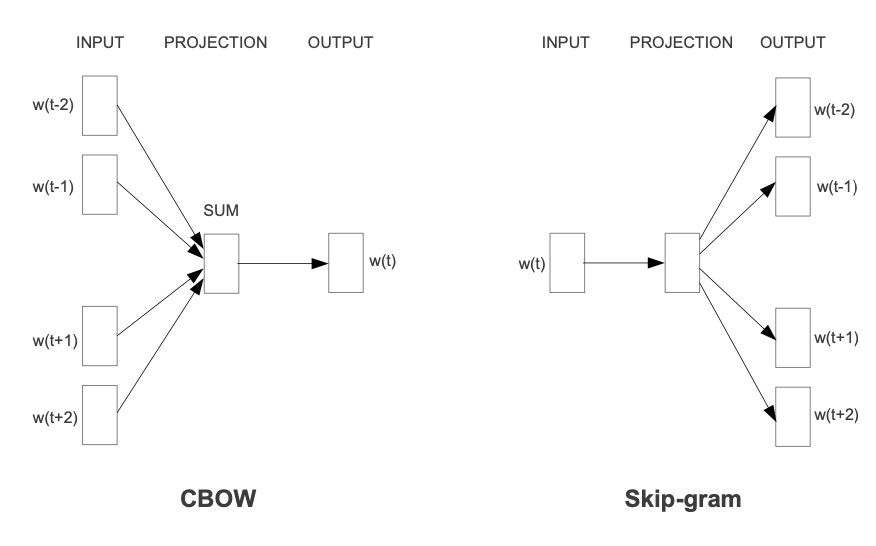
\includegraphics[scale=0.48]{figures/word2vec.png}
        \end{minipage}
        \begin{minipage}{0.4\textwidth}
        \textbf{ \;\;\; Documents as vectors} \\
        \begin{itemize}
            \setlength\itemsep{0em}
            \item Compute word embeddings
            \item Given a document and a query, compute their vector representations as average word embeddings (AWEs)
            \item Match using cosine similarity \\
        \end{itemize}
        \end{minipage}
        \item \textbf{\textcolor{PineGreen}{Document embeddings}}
        \begin{itemize}
            \item \textbf{Paragraph vector} \\
            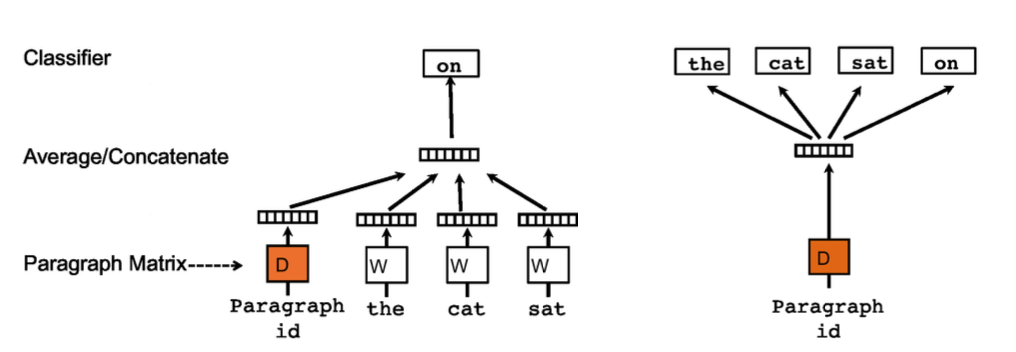
\includegraphics[scale=0.5]{figures/paragraph vector.png}
            
            \begin{minipage}{0.32\textwidth}
            \textbf{Paragraph vector} 
            \begin{itemize}
                \setlength\itemsep{0em}
                \item At every step of stochastic gradient descent, sample a fixed-length context from a random paragraph
                \item Compute the error gradient from the network
                \item Use the gradient to update parameters
            \end{itemize}
            \end{minipage}
            \begin{minipage}{0.58\textwidth}
            \textbf{ \;\;\; Documents as vectors} 
            \begin{itemize}
                \setlength\itemsep{0em}
                \item Compute document embeddings
                \item Given a query
                \begin{enumerate}
                    \setlength\itemsep{0em}
                    \item Fix the word matrix $W$
                    \item Add a (random) column to the document matrix $D$ corresponding to the query repr.
                    \item Update $D$ using gradient descent
                    \item Get the vector repr. of the query from the updated matrix $D$
                \end{enumerate}
                \item Match using cosine similarity
            \end{itemize}
            \end{minipage}
        \end{itemize}
    \end{itemize}
\end{enumerate}
